\chapter{Optimizing network-utilization by balancing workload}
\label{chap:balancing}

The last chapter brings an overview of different notations, algorithms and techniques.
In this chapter, all these instruments are combined to a chain for distributing routes more evenly.
The goal is to augment a given graph, such that diverse alternative paths can be found and used to spread the load (of a typical workload) while limiting the detours of individual \glspl{stpair}.
After the theory is explained, implementation-details are discussed.

For a given \gls{stpair} and a graph $G = (V, E)$ with vertices $V$ and edges $E$ of $d$-dimensional \glspl{weight}, a path should be found through an algorithm, that implicitly tends to distribute found paths over the network, while keeping the paths' \glspl{cost} sufficiently near every \gls{cost}-dimension's optimum.
To achieve this, a preprocessing-phase called \textit{balancing} analyzes the graph $G$ and computes a new \gls{metric}.
With this new \gls{metric}, routing-algorithms like \gls{dijkstra} \todo{TODO Check whether \gls{dijkstra} with \gls{personalized_routing} improves distribution with new metric or whether \gls{repr} is a must.} (with \gls{personalized_routing}) or like \gls{repr} can compute paths as usual.

It should be noted, that \gls{dijkstra} (bidirectional) instead of \gls{astar} is used for every occuring routing-query, may it be in \gls{repr} or anywhere else.
The reason is, that \gls{astar} works with heuristics, which are difficult to generalize over custom, artificial metrics.

\section{Preprocessing to create a new metric}

    \todo{both approaches: multiple runs (explicit euler because workload is toggling) vs multiple \glspl{metric}}
    \todo{normalization of all \glspl{metric} -> comparability between different graphs}

    This \textit{balancing} is depicted in figure~\ref{fig:balancing} and explained briefly in the caption or detailled in the following.

    \begin{figure}
        \centering
        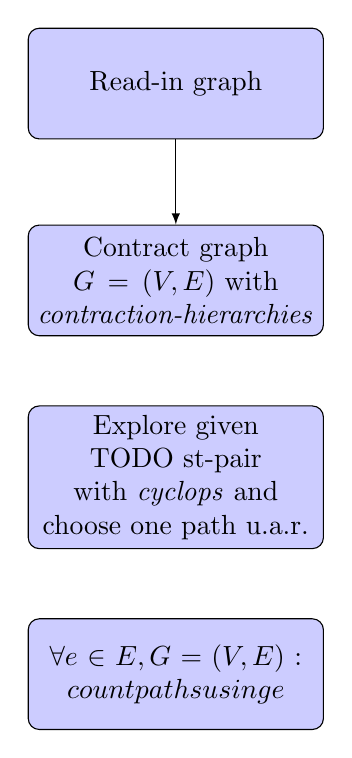
\begin{tikzpicture}[auto, rounded corners=0, node distance = 3cm, x=1cm, y=1cm] {%
    % style

    % draw
    % Draw borders

    % text badly centered
    % better use 'align=flush center'

    \tikzstyle{decision} = [%
        diamond,
        draw,
        fill = blue!20,
        text width = 4.5em,
        align = flush center,
        node distance = 3cm,
        inner sep = 0pt
    ]
    \tikzstyle{block} = [%
        rectangle,
        draw,
        fill = blue!20,
        text width = 10em,
        text centered,
        rounded corners,
        node distance = 2.5cm,
        minimum height = 4em
    ]
    \tikzstyle{cloud} = [%
        draw,
        ellipse,
        fill = red!20,
        node distance = 3cm,
        minimum height = 2em
    ]

    % arrow-styles
    % https://tex.stackexchange.com/questions/5461/is-it-possible-to-change-the-size-of-an-arrowhead-in-tikz-pgf
    \tikzstyle{line} = [draw, -latex]

    % Place nodes

    \node [block] (read-in_graph) {Read-in graph};
    \node [block, below of = read-in_graph] (contract_graph) {Contract graph $G=(V,E)$ with \textit{contraction-hierarchies}};
    \node [block, below of = contract_graph] (exploration) {Explore given TODO st-pair with \textit{cyclops} and choose one path u.a.r.};
    \node [block, below of = exploration] (analyzation) {$\forall e \in E, G = (V, E): count paths using e$};

    % Draw lines

    \path [line] (read-in_graph) -- (contract_graph);

    % \node [block] (init) {initialize model};
    % \node [cloud, left of=init] (expert) {expert};
    % \node [cloud, right of=init] (system) {system};

    % \node [block, below of=init] (identify) {identify candidate models};

    % \node [block, below of=identify] (evaluate) {evaluate candidate models};
    % \node [block, left of=evaluate, node distance=3cm] (update) {update model};

    % \node [decision, below of=evaluate] (decide) {is best candidate better?};

    % \node [block, below of=decide, node distance=3cm] (stop) {stop};

    % % Draw edges

    % \path [line] (init) -- (identify);
    % \path [line] (identify) -- (evaluate);
    % \path [line] (evaluate) -- (decide);
    % \path [line] (decide) -- node {no} (stop);

    % \path [line] (update) |- (identify);
    % \path [line] (decide) -| node [near start] {yes} (update);

    % \path [line,dashed] (expert) -- (init);
    % \path [line,dashed] (system) -- (init);
    % \path [line,dashed] (system) |- (evaluate);
} \end{tikzpicture}
        \caption[Overview of balancing a graph]{%
            This flow shows the balancer, that analyzes a given graph $G$.
            Shapes for actions are rectangular and blue, shapes for data are elliptical and red.
            A new, artificial \gls{metric} is created for $G$ and gets updated iteratively.
            It allows a routing-algorithm to distribute upcoming workload (like during rush-hour) more evenly over the underlying street-network.
            \label{fig:balancing}
        }
    \end{figure}

    \todo{TODO @Florian: Opinion about performance-issues below?}
    Let a graph $G = (V, E)$ of $d$ \glspl{metric} be given.
    For simplicity, all \glspl{metric} in $G$ are used for balancing and the \gls{personalized_routing} prefers all \glspl{metric} the same.
    Further, the set of \glspl{stpair}, which is used for balancing $G$, chooses $s$ and $t$ from $V$ \gls{uar}.
    Therefore, a sufficiently large set of \glspl{stpair} is needed to overload $G$.
    This clearly becomes a bottleneck for performance on larger graphs.
    On the other side, real, daily, critical \glspl{stpair} are not distributed \gls{uar} over $V$.
    The rush-hour in the morning, when everybody travels from their home to work, is a good counterexample here.
    The set of chosen $t$ might be much smaller than the number of $s$, and less people live near industry or motorways.
    Heuristics as described in~\cite{bakillah:population_from_osm} can return \glspl{stpair} based on approximating population-data from street-networks.
    So considering more specific sets of \glspl{stpair} might be interesting and helpful here, but is not covered in this thesis.

    At first, the graph $G$, that should be balanced, has to be read in, resulting in $G = (V, E)$ of $d$ \glspl{metric}.
    This graph $G$ is contracted via \gls{contraction-hierarchies} to $G_{CH}$.
    The step of contracting is not needed for correctness, but reduces the needed runtime (even if $G$ is not being fully contracted).

\section{Executing queries on the balanced graph}

    \todo{TODO write}

\section{Some implementation-details}
\label{chap:balancing:implementation}

    \todo{highlights, what was difficult/much work? -> repo-link}

    \subsection{Graphs and paths}

        \todo{TODO Write: Street-network as offset-graph (TODO: wrong name)}

        \todo{TODO Accessing the graph-structure}

    \subsection{Configs}

        \todo{TODO add some text here}
% - indices -> boost for performance while staying dynamic
% - Dijkstra, no A* because multiple metrics vs heuristic